%% Standalone lecture -- build with:  pdflatex -shell-escape matrixFactorisation
%% Shared preamble for standalone lecture files.
%%
%% Every lecture begins with %% Shared preamble for standalone lecture files.
%%
%% Every lecture begins with %% Shared preamble for standalone lecture files.
%%
%% Every lecture begins with \input{preamble} and is compiled on its own:
%%     pdflatex -shell-escape <lecture>
%% There is no master lectures.tex any more -- the list of lectures lives in
%% lectures.yaml and is read by the build scripts.

\documentclass[25pt,landscape,footrule]{foils}
\input{macros_gen}
\backgroundsetup{contents={}}

\usepackage{stmaryrd}
\usepackage{ifthen}
\usepackage{pdf14}

% Every figure lives in this course's lectures/figures (consolidated
% 2026-10-08).  Do not add other courses' folders back: when a name exists in
% several folders LaTeX silently takes the first, which mixed old and new
% frames of the same animation.  A missing figure should be a build error.
\graphicspath{{figures/}{../lectures/figures/}}

\date{}

\newcounter{lessoncnt}
\newcommand{\lesson}[1]{\setcounter{page}{1}%
\section{Mathematics of Machine Learning\\%
\vfill
\textcolor{red}{\textit{#1}}
\vfill}}
 and is compiled on its own:
%%     pdflatex -shell-escape <lecture>
%% There is no master lectures.tex any more -- the list of lectures lives in
%% lectures.yaml and is read by the build scripts.

\documentclass[25pt,landscape,footrule]{foils}
%\usepackage[compat2,pdftex]{geometry}
\usepackage[pdftex]{geometry}
\geometry{headsep=-2.5ex,hscale=0.9,bmargin=2.5cm,tmargin=1cm,textwidth=25cm}
\usepackage[pdftex]{xcolor}
\usepackage{pause}
\usepackage{background}
%\usepackage[color=white]{background}
\usepackage{listings}
\usepackage{graphicx}
\usepackage{epsfig}
\usepackage{epstopdf}
\usepackage{bm}
\usepackage{amssymb}
\usepackage{amsfonts}
\usepackage{marvosym}
\usepackage{cite}
\usepackage{pifont}
\usepackage[english]{babel}
\usepackage{amsmath}
\usepackage{amsfonts}
\usepackage{rotating}
\usepackage{listings}
\usepackage{pp4slide}
%\usepackage{hyperref}
\usepackage{pp4link}
\usepackage{fancyvrb}
\usepackage{multido}
\usepackage{calc}
\usepackage{mleftright}
\mleftright % Redefines \left to \mleft and \right to \mright



\thinmuskip=1mu

\newcommand{\bigstrut}{\rule[-0.5\baselineskip]{0pt}{1.2\baselineskip}}
\renewcommand{\ttdefault}{pcr}

\newcommand{\squeeze}{\setlength{\itemsep}{-2pt}}
%\renewcommand{\familydefault}{cmr}
%\renewcommand{\labelitemii}{\textcolor{green}{$\star$}}
\newcommand{\tick}{{\large \ding{51}}}
\newcommand{\cross}{{\large \ding{55}}}
%\DeclareMathAlphabet{\mat}{OT1}{cmss}{bx}{n}
\DeclareMathAlphabet{\mat}{U}{eur}{b}{n}
\newcommand{\figs}{/home/apb/figures}
\newcommand{\stimes}{{\scriptstyle \times}}
\newcommand{\tr}{\textsf{T}}
\newcommand{\e}[1]{{\rm e}^{#1}}
\newcommand{\E}[1]{{\rm e}^{{\displaystyle #1}}}
\newcommand{\av}[2][]{\mathbb{E}_{#1}\left[ #2 \right]}
\newcommand{\Var}[1]{\mathbb{V}\mathrm{ar}\left( #1 \right)}
\newcommand{\pred}[1]{\left\llbracket { \small #1} \right\rrbracket}
\newcommand{\logg}[1]{\log\left( #1 \right)}
\newcommand{\logtwo}[1]{\log_2\left( #1 \right)}
\newcommand{\bra}[1]{\left( #1 \right)}
\newcommand{\prob}[1]{\mathbb{P}\left( #1 \right)}
\newcommand{\Prob}[1]{\mathbb{P}\left( #1 \right)}
\newcommand{\Step}{\mathop{\mat{\Theta}}}
\newcommand\diag{\mathop{\mathrm{diag}}}
\newcommand{\grad}{\bm{\nabla}}
\newcommand{\gradx}{\bm{\nabla}_{\!\!\scriptscriptstyle \bm{x}}}
\newcommand{\gradw}{\bm{\nabla}_{\!\!\scriptscriptstyle \bm{w}}}
\newcommand{\dd}{\mathrm{d}}
\newcommand{\ii}{\mathrm{i}}
\newcommand{\data}{\mathcal{D}}
\newcommand{\class}{\mathcal{C}}
\newcommand{\hypo}{\mathcal{H}}
\newcommand{\indep}{\perp \!\!\!\! \perp}
\newcommand{\pd}[3][\,]{\frac{\partial^{#1}{#2}}{\partial\,{#3}}}
\newcommand{\normal}[1]{\mathcal{N}\!\left( #1 \right)}
\newcommand{\Dist}[2][Binom]{\mathrm{#1}\left( \strut {#2} \right)}
\newcommand{\brackets}[1]{\!\left( #1 \right)}
\newcommand{\KL}[2]{\mathop{\mathrm{KL}}\left(#1 \big\| #2\right)}
\newcommand{\argmax}{\mathop{\mathrm{argmax}}}
\newcommand{\argmin}{\mathop{\mathrm{argmin}}}
\newcommand{\margin}{\Delta}
\lstnewenvironment{matlab}[1][frame=TB]{\lstset{#1}}{}       
%\renewcommand{\emph}[1]{\textcolor{red}{\textbf{#1}}}
\newcommand{\myskip}[1]{}
\newcommand\mycom[2]{\genfrac{}{}{0pt}{}{#1}{#2}}
\newcommand{\jl}{\lstinline[basicstyle=\ttfamily\color{DarkGreen},%
 keywordstyle=\bfseries\ttfamily\color{DarkGreen}]}
\definecolor{EmphColor}{rgb}{0.0,0.0,1.0}
\renewcommand{\emph}[1]{{\color{EmphColor}\textbf{#1}}}
\newcommand{\len}[1]{\| #1 \|}
\newcommand{\inner}[2]{\left\langle {#1}, {#2}\right\rangle}
\newenvironment{psmallmatrix}{\left(\begin{smallmatrix}}{\end{smallmatrix}\right)}
  

\definecolor{DarkGreen}{rgb}{0,0.5,0}
\definecolor{DarkRed}{rgb}{0,0,0.5}
\definecolor{HighLight}{rgb}{1,0,0}     % yellow
\definecolor{TextColor}{rgb}{0.0,0.1,0.1}     % white
\definecolor{TwoColor}{rgb}{0.0,0.5,0.1}      % used for switching colors

\definecolor{HeadLineColor}{rgb}{1.0,0.0,0.0} % cyan
\definecolor{SpecialColor}{rgb}{0.53,0.81,1.0}
\renewcommand{\normalcolor}{\color{HeadLineColor}}

\pausecolors{TwoColor}{TextColor}{HighLight}
\pausecolors{EmphColor}{TextColor}{EmphColor}
\pausecolors{DarkGreen}{DarkGreen}{DarkRed}
\pausecolors{SpecialColor}{white}{HighLight}

\newenvironment{PauseHighLight}{\color{TwoColor}\pausehighlight}{}
\newcommand{\multipdf}[2][width=\linewidth]{\multiinclude[pause=\pauselevel{:+0}\pause,format=pdf,graphics={#1}]{#2}}

\lstdefinelanguage{pseudo}
 {keywords={all,and,begin,break,continue,do,else,elseif,%
     end,endif,endfor,endwhile,%
     exit,false,for,forall,goto,if,%
     or,return,then,true,to,repeat,until,while},%
  comment=[s]{/*}{*/},%
  morecomment=[l]//,%
  morestring=[d]"%
 }[keywords,comments,strings]


\lstloadlanguages{Java,pseudo,Python}
\lstset{
  basicstyle=\footnotesize\ttfamily\color{DarkGreen},
  keywordstyle=\bfseries\footnotesize\ttfamily\color{DarkGreen},
  commentstyle=\footnotesize\it\rmfamily\color{blue},
  language=Java,
  showstringspaces=false
  }


\lstnewenvironment{pseudo}[1][]{\lstset{language=pseudo,mathescape,literate={:=}{{$\gets$}}2 {!}{{$\neg$}}1 {!=}{{\!\!$\neq$\,\,}}2 {<=}{{\!\!$\leq$\,\,}}2 {>=}{{\!\!$\geq$\,\,}}2,escapechar=\#,#1}}{}
\lstnewenvironment{java}[1][]{\lstset{escapechar=\$,#1}}{}
% Python code: the language setting makes # comments use commentstyle.
% Comments stay monospaced: the default italic roman letter-spaces badly
% on listings' fixed columns.
\lstnewenvironment{python}[1][frame=TB]{\lstset{language=Python,
    commentstyle=\footnotesize\ttfamily\color{blue},#1}}{}

\MyLogo{}
%\Restriction{}
%\rightfooter{\hyperlink{overview}{$\square$}}

\newcommand{\keywords}[1]{\vfill{\noindent\it #1}}

\newcounter{outlineitem}
\setcounter{outlineitem}{0}
\newcommand{\outlineitem}[2]{\item%
  \def\targ{\value{emumi}}%
  \ifnum\value{enumi}=\value{outlineitem}%
  \color{HighLight}\textbf{#1}\toptarget{#2}\color{TextColor}%
   \else\toplink{#2}{#1}\fi
}
\color{TwoColor}


%-- Instead of writing \section we want the file structured by \section.
\newcommand{\section}[2][0]{\foilhead[#1cm]{#2}}

%-- Write each page into a \begin{slide} -- \end{slide} environment.
\newenvironment{slide}{}{\pauselevel{=1}}

\MyLogo{\pauselevel{=1}\Acrobatmenu{GoBack}{%
  \color{TextColor}{Adam Pr\"ugel-Bennett}} \hspace{2cm}
  % Clicking on the name steps one slide back.
  \toplink{firstoutline}{\color{red}Mathematics of Machine
    Learning}%
  \hspace{2cm}
  \texttt{//ecs-vlc.github.io/aice3001/}
  %Clicking on the date jumps to the last page, which should be the
  %table of contents.
  \rightfooter{\Acrobatmenu{LastPage}{\qquad%
  \textsf{\color{TextColor}\tiny\thepage}}}% page number
  % Clicking on the page number steps one slide back.
}
\raggedright
\newcommand{\Outline}{}

\newcommand{\pb}{\pausebuild \color{TwoColor}}
\newcommand{\pauseb}{\pauselevel{build, highlight}\pause}
\newcommand{\hl}[1]{\pauselevel{=1, highlight =1 :1, highlight =#1 :#1}\pause}
\newcommand{\hll}{\pauselevel{=1, highlight =1 :1}\pause}
\newcommand{\pauseh}{\pauselevel{highlight}\pause}
\newcommand{\nhl}[1]{\textcolor{TextColor}{#1}}
\newcommand{\mypl}[1]{\pauselevel{=#1 :#1}\pause}
\input supp-pdf.tex
\DeclareGraphicsRule{*}{mps}{*}{}
\usepackage{mpmulti}
%\leftheader{}
\rightheader{} % no more page numbers on top right


\hypersetup{pdftitle={ECS Lectures},pdfsubject={Machine Learning}
pdfauthor={Adam Prugel-Bennett},pdfkeywords={machine learning},
pdfpagemode={FullScreen},
bookmarksopen=false,
hypertexnames=false,pdfstartview={FitV},colorlinks,linkcolor={blue},
citecolor={green},urlcolor={blue}}



\newcommand\bluepage{
\clearpage
\renewcommand\normalcolor{\color{yellow}}
\pagecolor{blue}
\renewcommand\Black{\color{white}}
\color{white}
\hypersetup{colorlinks=true}
}

\newcommand\whitepage{
\clearpage
\renewcommand\normalcolor{\color{black}}
\pagecolor{white}
\renewcommand\Black{\color{black}}
\color{black}
\hypersetup{colorlinks=true}
}

\whitepage
\setlength{\unitlength}{1mm}

\newenvironment{leftImage}[2][0.3]{%
\begin{minipage}{#1\linewidth}
  \includegraphics[width=\linewidth]{#2}
\end{minipage}\hfill
\begin{minipage}{0.92\linewidth - #1\linewidth}}%
{\end{minipage}}

\newenvironment{rightImage}[2][0.3]{%
\newcommand{\foot}{\begin{minipage}{#1\linewidth}\includegraphics[width=0.98\linewidth]{#2}\end{minipage}}%
\begin{minipage}{0.95\linewidth - #1\linewidth}\raggedright }{\end{minipage}\hfill\foot}


%%% Local Variables: 
%%% mode: latex
%%% TeX-master: t
%%% End: 

\backgroundsetup{contents={}}

\usepackage{stmaryrd}
\usepackage{ifthen}
\usepackage{pdf14}

% Every figure lives in this course's lectures/figures (consolidated
% 2026-10-08).  Do not add other courses' folders back: when a name exists in
% several folders LaTeX silently takes the first, which mixed old and new
% frames of the same animation.  A missing figure should be a build error.
\graphicspath{{figures/}{../lectures/figures/}}

\date{}

\newcounter{lessoncnt}
\newcommand{\lesson}[1]{\setcounter{page}{1}%
\section{Mathematics of Machine Learning\\%
\vfill
\textcolor{red}{\textit{#1}}
\vfill}}
 and is compiled on its own:
%%     pdflatex -shell-escape <lecture>
%% There is no master lectures.tex any more -- the list of lectures lives in
%% lectures.yaml and is read by the build scripts.

\documentclass[25pt,landscape,footrule]{foils}
%\usepackage[compat2,pdftex]{geometry}
\usepackage[pdftex]{geometry}
\geometry{headsep=-2.5ex,hscale=0.9,bmargin=2.5cm,tmargin=1cm,textwidth=25cm}
\usepackage[pdftex]{xcolor}
\usepackage{pause}
\usepackage{background}
%\usepackage[color=white]{background}
\usepackage{listings}
\usepackage{graphicx}
\usepackage{epsfig}
\usepackage{epstopdf}
\usepackage{bm}
\usepackage{amssymb}
\usepackage{amsfonts}
\usepackage{marvosym}
\usepackage{cite}
\usepackage{pifont}
\usepackage[english]{babel}
\usepackage{amsmath}
\usepackage{amsfonts}
\usepackage{rotating}
\usepackage{listings}
\usepackage{pp4slide}
%\usepackage{hyperref}
\usepackage{pp4link}
\usepackage{fancyvrb}
\usepackage{multido}
\usepackage{calc}
\usepackage{mleftright}
\mleftright % Redefines \left to \mleft and \right to \mright



\thinmuskip=1mu

\newcommand{\bigstrut}{\rule[-0.5\baselineskip]{0pt}{1.2\baselineskip}}
\renewcommand{\ttdefault}{pcr}

\newcommand{\squeeze}{\setlength{\itemsep}{-2pt}}
%\renewcommand{\familydefault}{cmr}
%\renewcommand{\labelitemii}{\textcolor{green}{$\star$}}
\newcommand{\tick}{{\large \ding{51}}}
\newcommand{\cross}{{\large \ding{55}}}
%\DeclareMathAlphabet{\mat}{OT1}{cmss}{bx}{n}
\DeclareMathAlphabet{\mat}{U}{eur}{b}{n}
\newcommand{\figs}{/home/apb/figures}
\newcommand{\stimes}{{\scriptstyle \times}}
\newcommand{\tr}{\textsf{T}}
\newcommand{\e}[1]{{\rm e}^{#1}}
\newcommand{\E}[1]{{\rm e}^{{\displaystyle #1}}}
\newcommand{\av}[2][]{\mathbb{E}_{#1}\left[ #2 \right]}
\newcommand{\Var}[1]{\mathbb{V}\mathrm{ar}\left( #1 \right)}
\newcommand{\pred}[1]{\left\llbracket { \small #1} \right\rrbracket}
\newcommand{\logg}[1]{\log\left( #1 \right)}
\newcommand{\logtwo}[1]{\log_2\left( #1 \right)}
\newcommand{\bra}[1]{\left( #1 \right)}
\newcommand{\prob}[1]{\mathbb{P}\left( #1 \right)}
\newcommand{\Prob}[1]{\mathbb{P}\left( #1 \right)}
\newcommand{\Step}{\mathop{\mat{\Theta}}}
\newcommand\diag{\mathop{\mathrm{diag}}}
\newcommand{\grad}{\bm{\nabla}}
\newcommand{\gradx}{\bm{\nabla}_{\!\!\scriptscriptstyle \bm{x}}}
\newcommand{\gradw}{\bm{\nabla}_{\!\!\scriptscriptstyle \bm{w}}}
\newcommand{\dd}{\mathrm{d}}
\newcommand{\ii}{\mathrm{i}}
\newcommand{\data}{\mathcal{D}}
\newcommand{\class}{\mathcal{C}}
\newcommand{\hypo}{\mathcal{H}}
\newcommand{\indep}{\perp \!\!\!\! \perp}
\newcommand{\pd}[3][\,]{\frac{\partial^{#1}{#2}}{\partial\,{#3}}}
\newcommand{\normal}[1]{\mathcal{N}\!\left( #1 \right)}
\newcommand{\Dist}[2][Binom]{\mathrm{#1}\left( \strut {#2} \right)}
\newcommand{\brackets}[1]{\!\left( #1 \right)}
\newcommand{\KL}[2]{\mathop{\mathrm{KL}}\left(#1 \big\| #2\right)}
\newcommand{\argmax}{\mathop{\mathrm{argmax}}}
\newcommand{\argmin}{\mathop{\mathrm{argmin}}}
\newcommand{\margin}{\Delta}
\lstnewenvironment{matlab}[1][frame=TB]{\lstset{#1}}{}       
%\renewcommand{\emph}[1]{\textcolor{red}{\textbf{#1}}}
\newcommand{\myskip}[1]{}
\newcommand\mycom[2]{\genfrac{}{}{0pt}{}{#1}{#2}}
\newcommand{\jl}{\lstinline[basicstyle=\ttfamily\color{DarkGreen},%
 keywordstyle=\bfseries\ttfamily\color{DarkGreen}]}
\definecolor{EmphColor}{rgb}{0.0,0.0,1.0}
\renewcommand{\emph}[1]{{\color{EmphColor}\textbf{#1}}}
\newcommand{\len}[1]{\| #1 \|}
\newcommand{\inner}[2]{\left\langle {#1}, {#2}\right\rangle}
\newenvironment{psmallmatrix}{\left(\begin{smallmatrix}}{\end{smallmatrix}\right)}
  

\definecolor{DarkGreen}{rgb}{0,0.5,0}
\definecolor{DarkRed}{rgb}{0,0,0.5}
\definecolor{HighLight}{rgb}{1,0,0}     % yellow
\definecolor{TextColor}{rgb}{0.0,0.1,0.1}     % white
\definecolor{TwoColor}{rgb}{0.0,0.5,0.1}      % used for switching colors

\definecolor{HeadLineColor}{rgb}{1.0,0.0,0.0} % cyan
\definecolor{SpecialColor}{rgb}{0.53,0.81,1.0}
\renewcommand{\normalcolor}{\color{HeadLineColor}}

\pausecolors{TwoColor}{TextColor}{HighLight}
\pausecolors{EmphColor}{TextColor}{EmphColor}
\pausecolors{DarkGreen}{DarkGreen}{DarkRed}
\pausecolors{SpecialColor}{white}{HighLight}

\newenvironment{PauseHighLight}{\color{TwoColor}\pausehighlight}{}
\newcommand{\multipdf}[2][width=\linewidth]{\multiinclude[pause=\pauselevel{:+0}\pause,format=pdf,graphics={#1}]{#2}}

\lstdefinelanguage{pseudo}
 {keywords={all,and,begin,break,continue,do,else,elseif,%
     end,endif,endfor,endwhile,%
     exit,false,for,forall,goto,if,%
     or,return,then,true,to,repeat,until,while},%
  comment=[s]{/*}{*/},%
  morecomment=[l]//,%
  morestring=[d]"%
 }[keywords,comments,strings]


\lstloadlanguages{Java,pseudo,Python}
\lstset{
  basicstyle=\footnotesize\ttfamily\color{DarkGreen},
  keywordstyle=\bfseries\footnotesize\ttfamily\color{DarkGreen},
  commentstyle=\footnotesize\it\rmfamily\color{blue},
  language=Java,
  showstringspaces=false
  }


\lstnewenvironment{pseudo}[1][]{\lstset{language=pseudo,mathescape,literate={:=}{{$\gets$}}2 {!}{{$\neg$}}1 {!=}{{\!\!$\neq$\,\,}}2 {<=}{{\!\!$\leq$\,\,}}2 {>=}{{\!\!$\geq$\,\,}}2,escapechar=\#,#1}}{}
\lstnewenvironment{java}[1][]{\lstset{escapechar=\$,#1}}{}
% Python code: the language setting makes # comments use commentstyle.
% Comments stay monospaced: the default italic roman letter-spaces badly
% on listings' fixed columns.
\lstnewenvironment{python}[1][frame=TB]{\lstset{language=Python,
    commentstyle=\footnotesize\ttfamily\color{blue},#1}}{}

\MyLogo{}
%\Restriction{}
%\rightfooter{\hyperlink{overview}{$\square$}}

\newcommand{\keywords}[1]{\vfill{\noindent\it #1}}

\newcounter{outlineitem}
\setcounter{outlineitem}{0}
\newcommand{\outlineitem}[2]{\item%
  \def\targ{\value{emumi}}%
  \ifnum\value{enumi}=\value{outlineitem}%
  \color{HighLight}\textbf{#1}\toptarget{#2}\color{TextColor}%
   \else\toplink{#2}{#1}\fi
}
\color{TwoColor}


%-- Instead of writing \section we want the file structured by \section.
\newcommand{\section}[2][0]{\foilhead[#1cm]{#2}}

%-- Write each page into a \begin{slide} -- \end{slide} environment.
\newenvironment{slide}{}{\pauselevel{=1}}

\MyLogo{\pauselevel{=1}\Acrobatmenu{GoBack}{%
  \color{TextColor}{Adam Pr\"ugel-Bennett}} \hspace{2cm}
  % Clicking on the name steps one slide back.
  \toplink{firstoutline}{\color{red}Mathematics of Machine
    Learning}%
  \hspace{2cm}
  \texttt{//ecs-vlc.github.io/aice3001/}
  %Clicking on the date jumps to the last page, which should be the
  %table of contents.
  \rightfooter{\Acrobatmenu{LastPage}{\qquad%
  \textsf{\color{TextColor}\tiny\thepage}}}% page number
  % Clicking on the page number steps one slide back.
}
\raggedright
\newcommand{\Outline}{}

\newcommand{\pb}{\pausebuild \color{TwoColor}}
\newcommand{\pauseb}{\pauselevel{build, highlight}\pause}
\newcommand{\hl}[1]{\pauselevel{=1, highlight =1 :1, highlight =#1 :#1}\pause}
\newcommand{\hll}{\pauselevel{=1, highlight =1 :1}\pause}
\newcommand{\pauseh}{\pauselevel{highlight}\pause}
\newcommand{\nhl}[1]{\textcolor{TextColor}{#1}}
\newcommand{\mypl}[1]{\pauselevel{=#1 :#1}\pause}
\input supp-pdf.tex
\DeclareGraphicsRule{*}{mps}{*}{}
\usepackage{mpmulti}
%\leftheader{}
\rightheader{} % no more page numbers on top right


\hypersetup{pdftitle={ECS Lectures},pdfsubject={Machine Learning}
pdfauthor={Adam Prugel-Bennett},pdfkeywords={machine learning},
pdfpagemode={FullScreen},
bookmarksopen=false,
hypertexnames=false,pdfstartview={FitV},colorlinks,linkcolor={blue},
citecolor={green},urlcolor={blue}}



\newcommand\bluepage{
\clearpage
\renewcommand\normalcolor{\color{yellow}}
\pagecolor{blue}
\renewcommand\Black{\color{white}}
\color{white}
\hypersetup{colorlinks=true}
}

\newcommand\whitepage{
\clearpage
\renewcommand\normalcolor{\color{black}}
\pagecolor{white}
\renewcommand\Black{\color{black}}
\color{black}
\hypersetup{colorlinks=true}
}

\whitepage
\setlength{\unitlength}{1mm}

\newenvironment{leftImage}[2][0.3]{%
\begin{minipage}{#1\linewidth}
  \includegraphics[width=\linewidth]{#2}
\end{minipage}\hfill
\begin{minipage}{0.92\linewidth - #1\linewidth}}%
{\end{minipage}}

\newenvironment{rightImage}[2][0.3]{%
\newcommand{\foot}{\begin{minipage}{#1\linewidth}\includegraphics[width=0.98\linewidth]{#2}\end{minipage}}%
\begin{minipage}{0.95\linewidth - #1\linewidth}\raggedright }{\end{minipage}\hfill\foot}


%%% Local Variables: 
%%% mode: latex
%%% TeX-master: t
%%% End: 

\backgroundsetup{contents={}}

\usepackage{stmaryrd}
\usepackage{ifthen}
\usepackage{pdf14}

% Every figure lives in this course's lectures/figures (consolidated
% 2026-10-08).  Do not add other courses' folders back: when a name exists in
% several folders LaTeX silently takes the first, which mixed old and new
% frames of the same animation.  A missing figure should be a build error.
\graphicspath{{figures/}{../lectures/figures/}}

\date{}

\newcounter{lessoncnt}
\newcommand{\lesson}[1]{\setcounter{page}{1}%
\section{Mathematics of Machine Learning\\%
\vfill
\textcolor{red}{\textit{#1}}
\vfill}}


\begin{document}

\lesson{Matrix Factorisation}
\vspace{-1cm}
\begin{center}
    \begin{tabular}{|l||c|c|c|c|c|}\hline
      Name & Titanic & Dr No & The Matrix & Spartacus & Ten \\ \hline
      Alice & 2 & \O & 4  & 5 & 2  \\ \hline
      Bob   & 5 & 3  & \O & 3 & \O \\ \hline
      Chas  & \O & 2 & 3 & 5 & 3 \\ \hline
    \end{tabular}
\end{center}
\keywords{Matrix completion, low-rank approximation, recommender systems, alternating least squares, non-negative matrix factorisation}
%%%%%%%%%%%%%%%%%%%%%%% Next Slide %%%%%%%%%%%%%%%%%%%%%%%
\renewcommand{\Outline}{%
\begin{slide}
\section[1]{Outline}

\begin{minipage}{12cm}\raggedright
  \begin{enumerate}
    \outlineitem{Missing Data and Recommenders}{recommenders}
    \outlineitem{Low-Rank Approximation}{lowrank}
    \outlineitem{Probabilistic Approach}{prob}
    \outlineitem{Non-Negative Matrix Factorisation}{nnmf}
  \end{enumerate}
\end{minipage}\hfill
\begin{minipage}{10cm}
  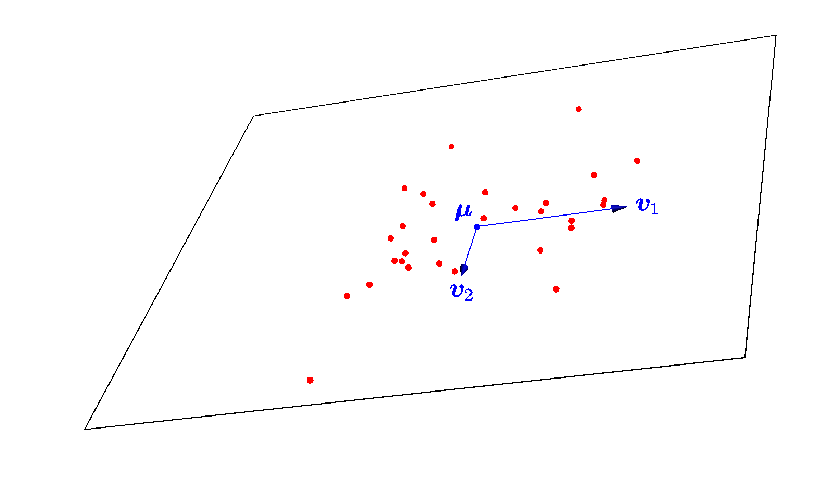
\includegraphics[width=10cm]{lowrank-3}
\end{minipage}
\end{slide}
\addtocounter{outlineitem}{1}
}

\setcounter{outlineitem}{1}

%%%%%%%%%%%%%%%%%%%%%%% Next Slide %%%%%%%%%%%%%%%%%%%%%%%
\Outline % Missing Data and Recommenders
\toptarget{firstoutline}
%%%%%%%%%%%%%%%%%%%%%%% Next Slide %%%%%%%%%%%%%%%%%%%%%%%

\begin{slide}
\section{Matrix Completion}

\begin{PauseHighLight}
  \begin{itemize}
  \item It is extremely common to be given a matrix of data with
    missing entries\pause{} (particularly when the data comes from
    humans filling in forms)\pause
  \item Most learning machines need a complete set of data, so we
    either throw away examples or features with missing values
    (sometimes leaving nothing) or do our best to infer them\pause
  \item Inferring them only works if there is structure in the matrix
    that we can exploit\pause
  \item The structure we use in this lecture: \emph{structured data
      typically lies close to a low-dimensional subspace}\pause{}
    (the idea behind PCA and the SVD)\pause
  \end{itemize}
\end{PauseHighLight}

\end{slide}

%%%%%%%%%%%%%%%%%%%%%%% Next Slide %%%%%%%%%%%%%%%%%%%%%%%

\begin{slide}
\section{Recommender Systems}

\begin{PauseHighLight}
\begin{itemize}\squeeze
\item The best-known example: recommending items to users, which can
  be financially important
  \begin{itemize}
  \item Recommendations are reported to drive a large share of
    Amazon's sales\pause
  \item Netflix (then a DVD rental company, now a streaming service)
    ran a \$1 million competition (2006--09) to improve the quality of
    its recommendations\pause
  \end{itemize}
\item \emph{Content-based filtering} uses (often text) features to
  find similar items; \emph{collaborative filtering} uses ratings
  supplied (implicitly or explicitly) by users\pause
\item We concentrate on collaborative filtering\pause
\end{itemize}
\end{PauseHighLight}
\end{slide}

%%%%%%%%%%%%%%%%%%%%%%% Next Slide %%%%%%%%%%%%%%%%%%%%%%%

\begin{slide}
\section[-2]{Recommending Movies}

\begin{PauseHighLight}
  \begin{itemize}
  \item The classic example is to recommend a movie given some ratings
    from users
    \begin{center}
    \begin{tabular}{|l||c|c|c|c|c|}\hline
      Name & Titanic & Dr No & The Matrix & Spartacus & Ten \\ \hline
      Alice & 2 & \O & 4  & 5 & 2  \\ \hline
      Bob   & 5 & 3  & \O & 3 & \O \\ \hline
      Chas  & \O & 2 & 3 & 5 & 3 \\ \hline
    \end{tabular}\pause
    \end{center}
  \item \O\ means there are no ratings\pause
  \item The task is to predict the unknown ratings and make a
    recommendation\pause
  \item Typically data sets are huge and very sparse\pause
  \end{itemize}
\end{PauseHighLight}

\end{slide}

%%%%%%%%%%%%%%%%%%%%%%% Next Slide %%%%%%%%%%%%%%%%%%%%%%%

\begin{slide}
\section{Classic Collaborative Filtering}

\begin{PauseHighLight}
  \begin{minipage}{0.58\linewidth}
    \begin{itemize}
    \item The classic collaborative filtering technique is to find similar
      users (those giving similar ratings)\pause
    \item Use the recommendation of similar users weighted by
      their similarity\pause
    \item Can also recommend items that are similar (i.e. items
      that have received similar ratings) to those that a user rates
      highly\pause
    \end{itemize}
  \end{minipage}\hfil
\begin{minipage}{0.40\linewidth}
  \begin{center}
    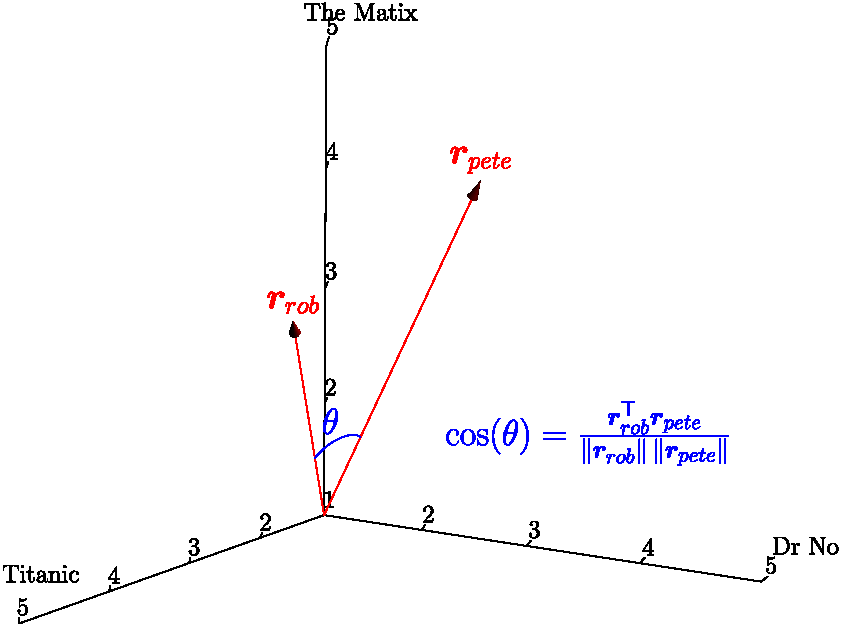
\includegraphics[width=\linewidth]{cosineSim}
  \end{center}
  \pauselevel{=2}
  \begin{align*}
    \hat{R}_{ui} = \frac{\sum\limits_{u'} \mathrm{sim}(u,u')\,
    R_{u'i}}{\sum\limits_{u'} \mathrm{sim}(u,u')}\pause
  \end{align*}
\end{minipage}
\end{PauseHighLight}

\end{slide}


%%%%%%%%%%%%%%%%%%%%%%% Next Slide %%%%%%%%%%%%%%%%%%%%%%%
\Outline % Low Rank
%%%%%%%%%%%%%%%%%%%%%%% Next Slide %%%%%%%%%%%%%%%%%%%%%%%

\begin{slide}
\section[-1]{Matrix Completion}

\begin{PauseHighLight}
  \begin{itemize}
  \item A different (often better) method is to think of recommendation
    as a matrix completion task
    \begin{center}
    \begin{tabular}{|l||c|c|c|c|c|}\hline
      Name & Titanic & Dr No & The Matrix & Spartacus & Ten \\ \hline
      Alice & 2 & \O & 4  & 5 & 2  \\ \hline
      Bob   & 5 & 3  & \O & 3 & \O \\ \hline
      Chas  & \O & 2 & 3 & 5 & 3 \\ \hline
    \end{tabular}\pause
    \end{center}
  \item Complete the matrix
    \begin{align*} \mat{R} =
      \begin{pmatrix}
        2& & 4 & 5 & 2  \\
        5 & 3  &   & 3 &   \\
          & 2 & 3 & 5 & 3
      \end{pmatrix}
    \end{align*}\pause
  \end{itemize}
\end{PauseHighLight}

\end{slide}

%%%%%%%%%%%%%%%%%%%%%%% Next Slide %%%%%%%%%%%%%%%%%%%%%%%

\begin{slide}
\section[-1]{Replace by Means}

\begin{PauseHighLight}
  \begin{itemize}\squeeze
  \item The simplest guess uses the means, column-wise and row-wise
    \begin{align*}
      R_{ui} \approx \bar{R}_u + \bar{R}_i - \bar{R}
    \end{align*}
    where
    \begin{itemize}
    \item $\bar{R}_u$ is the mean rating of user $u$
    \item $\bar{R}_i$ is the mean rating for item $i$
    \item $\bar{R}$ is the mean overall rating\pause
    \end{itemize}
  \item Gets the means right and gives a reasonable rating\pause
  \item (For general missing data: replace by the feature's mean)\pause
  \item But this ignores structure: similar users give similar
    ratings\pause
  \end{itemize}
\end{PauseHighLight}

\end{slide}

%%%%%%%%%%%%%%%%%%%%%%% Next Slide %%%%%%%%%%%%%%%%%%%%%%%

\begin{slide}
\section[-2]{Best Low-Rank Approximation}

\begin{PauseHighLight}
  \begin{itemize}\squeeze
  \item Recall the SVD of a complete matrix, with
    $s_1\geq s_2\geq\cdots\geq0$
    \begin{align*}
      \mat{X} = \mat{U}\,\mat{S}\,\mat{V}^\tr = \sum_k s_k\,
      \bm{u}_k\,\bm{v}_k^\tr\pause
    \end{align*}
  \item Keeping the $K$ largest singular values gives a rank-$K$
    matrix $\mat{X}_K = \sum_{k=1}^K s_k\, \bm{u}_k\,\bm{v}_k^\tr$\pause
  \item \emph{Eckart--Young theorem}: $\mat{X}_K$ is the best rank-$K$
    approximation to $\mat{X}$, with error
    $\|\mat{X}-\mat{X}_K\|_F^2 = \sum_{k>K} s_k^2$\pause{} (also best in
    the spectral norm, with error $s_{K+1}$)\pause
  \item Data close to a $K$-dimensional subspace has small discarded
    $s_k$\pause{} (this is effectively PCA)\pause
  \end{itemize}
\end{PauseHighLight}

\end{slide}

%%%%%%%%%%%%%%%%%%%%%%% Next Slide %%%%%%%%%%%%%%%%%%%%%%%

\begin{slide}
\section[-1]{Completing a Matrix with the SVD}

\begin{PauseHighLight}
  \begin{itemize}
  \item The SVD needs a complete matrix, so we iterate\pause
    \begin{enumerate}
    \item Fill in the missing entries (e.g. with the user means)\pause
    \item Compute the best rank-$K$ approximation $\mat{L}$ of the
      filled-in matrix\pause
    \item Replace the missing entries (only) by the values in
      $\mat{L}$\pause
    \item Repeat from 2\pause
    \end{enumerate}
  \item With a mask $\mat{W}$ ($W_{ij}=1$ where $X_{ij}$ is observed,
    $0$ otherwise) and $\odot$ the element-by-element product
    \begin{align*}
      \mat{X}(t+1) = \mat{W}\odot\mat{X} + \overline{\mat{W}}\odot
      \mat{L}(t)
    \end{align*}
    where $\overline{\mat{W}} = 1 - \mat{W}$\pause
  \end{itemize}
\end{PauseHighLight}

\end{slide}

%%%%%%%%%%%%%%%%%%%%%%% Next Slide %%%%%%%%%%%%%%%%%%%%%%%

\begin{slide}
\section{SVD in Operation}
\pause
\pb
\pauselevel{=1}
\begin{center}
  \multipdf[width=0.95\linewidth]{svdComplete}\pause
\end{center}
\end{slide}

%%%%%%%%%%%%%%%%%%%%%%% Next Slide %%%%%%%%%%%%%%%%%%%%%%%

\begin{slide}
\section{Low-Rank Approximation}

\begin{PauseHighLight}
  \begin{itemize}
  \item More directly, approximate an $m\times n$ matrix $\mat{X}$ by
    \begin{align*}
      \mat{X} \approx \mat{A}\; \mat{B}
    \end{align*}
    where $\mat{A}$ is $m \times K$ and $\mat{B}$ is
    $K\times n$\pause
  \item $\mat{A} \mat{B}$ has \textit{rank} at most $K$\pause
  \item We replace $m\times n$ elements by $(m+n)\times K$ free
    parameters\pause
  \item $K$ controls the complexity of the model: large $K$ fits the
    data better but may over-fit\pause
  \item Choose $K$ by cross-validation (hide some of the observed
    entries and see how well we predict them)\pause
  \end{itemize}
\end{PauseHighLight}

\end{slide}

%%%%%%%%%%%%%%%%%%%%%%% Next Slide %%%%%%%%%%%%%%%%%%%%%%%

\begin{slide}
\section[-2]{Low-Rank Updates: LoRA}

\begin{PauseHighLight}\squeeze
  \begin{itemize}
  \item \emph{LoRA} (low-rank adaptation, Hu et al.\ 2021) uses the same
    idea to fine-tune a large network: a pretrained weight matrix
    $\mat{W}_0$ ($m\times n$) becomes $\mat{W}_0 + \Delta\mat{W}$\pause
  \item LoRA freezes $\mat{W}_0$ and learns only a low-rank change
    \begin{align*}
      \Delta\mat{W} = \mat{A}\,\mat{B}, \qquad \mat{A}\ (m\times K),\
      \mat{B}\ (K\times n),\ K\ll m,n\pause
    \end{align*}
    with one factor starting at zero (so training starts from
    $\mat{W}_0$)\pause
  \item For $m=n=4096$ and $K=8$: $(m+n)K \approx 6.6\times10^4$
    parameters to train instead of $mn\approx1.7\times10^7$ (0.4\%)\pause
  \item The bet: the change a new task needs is close to low rank;\pause{}
    each task stores only its own $\mat{A}$, $\mat{B}$, and $\mat{A}\mat{B}$
    can be added into $\mat{W}_0$ afterwards\pause
  \end{itemize}
\end{PauseHighLight}

\end{slide}

%%%%%%%%%%%%%%%%%%%%%%% Next Slide %%%%%%%%%%%%%%%%%%%%%%%

\begin{slide}
\section{Least-Squares}

\begin{PauseHighLight}
  \begin{itemize}
  \item Assume we have elements of $\mat{X}$ only at the locations
    $\mathcal{D}$\pause
  \item We can seek a least-squares solution for $\mat{A}$ and $\mat{B}$
    \begin{align*}
      (\mat{A},\mat{B}) = \mathop{\mathrm{argmin}}\limits_{(\mat{A},\mat{B})}
      \sum_{(i,j)\in\mathcal{D}} \left( X_{ij} -
        \sum_{k=1}^K A_{ik} \, B_{kj} \right)^2\pause
    \end{align*}
  \item OK, but it can over-fit\pause
  \item $\mat{A}$ and $\mat{B}$ are never unique:
    $\mat{A}\mat{B} = (\mat{A}\mat{G})(\mat{G}^{-1}\mat{B})$ for any
    invertible $K\times K$ matrix $\mat{G}$\pause
  \end{itemize}
\end{PauseHighLight}

\end{slide}

%%%%%%%%%%%%%%%%%%%%%%% Next Slide %%%%%%%%%%%%%%%%%%%%%%%
\Outline % Probabilistic Approach
%%%%%%%%%%%%%%%%%%%%%%% Next Slide %%%%%%%%%%%%%%%%%%%%%%%

\begin{slide}
\section[-2]{Bayes' Rule and MAP}

\begin{PauseHighLight}
  \begin{itemize}\squeeze
  \item For parameters $\bm{\theta}$ and data $\data$, Bayes' rule
    gives the \emph{posterior} (likelihood $\times$ prior $/$ evidence)
    \begin{align*}
      \Prob{\bm{\theta}|\data} =
      \frac{\Prob{\data|\bm{\theta}}\,\Prob{\bm{\theta}}}{\Prob{\data}}\pause
    \end{align*}
  \item The \emph{maximum a posteriori} (MAP) solution is the most
    probable $\bm{\theta}$ ($\Prob{\data}$ does not depend on it)
    \begin{align*}
      \bm{\theta}_{\mathrm{MAP}} = \mathop{\mathrm{argmax}}_{\bm{\theta}}
      \Bigl(\logg{\Prob{\data|\bm{\theta}}} + \logg{\Prob{\bm{\theta}}}\Bigr)\pause
    \end{align*}
  \item With a flat prior it is the maximum-likelihood solution\pause
  \item Limitations: MAP gives a single point, throwing away our
    uncertainty about $\bm{\theta}$;\pause{} and the peak of a density
    depends on how we parametrise $\bm{\theta}$\pause
  \end{itemize}
\end{PauseHighLight}

\end{slide}

%%%%%%%%%%%%%%%%%%%%%%% Next Slide %%%%%%%%%%%%%%%%%%%%%%%

\begin{slide}
\section{Bayesian Approach}

\begin{PauseHighLight}
  \begin{itemize}
  \item We can use a Bayesian approach to infer $\mat{A}$ and $\mat{B}$\pause
  \item The likelihood is
    \begin{align*}
      \Prob{X_{ij}|\mat{A},\mat{B}} &=
      \mathcal{N}\left(X_{ij}\bigg|\sum_{k=1}^K
        A_{ik} \, B_{kj}, \sigma^2\right) \\
      \mathcal{N}(x|\mu,\sigma^2) &= \frac{1}{\sqrt{2\,\pi\,}\;\sigma}
      \e{-(x-\mu)^2/(2\,\sigma^2)}
    \end{align*}
  \item $\sigma$ measures the natural error in the ratings\pause
  \end{itemize}
\end{PauseHighLight}

\end{slide}

%%%%%%%%%%%%%%%%%%%%%%% Next Slide %%%%%%%%%%%%%%%%%%%%%%%

\begin{slide}
\section{Priors}

\begin{PauseHighLight}
  \begin{itemize}
  \item We also need priors
    \begin{align*}
      \Prob{\mat{A}} &= \prod_{i,k} \mathcal{N}(A_{ik}|0,\sigma_A^2), &
      \Prob{\mat{B}} &= \prod_{k,j} \mathcal{N}(B_{kj}|0,\sigma_B^2) \pause
    \end{align*}
  \item $\sigma_A^2$ and $\sigma_B^2$ explain the variation in the
    original matrix $\mat{X}$\pause
  \item Note that
    \begin{align*}
      \av{\sum_{k=1}^K A_{ik} \, B_{kj}} &= 0, &
      \Var{\sum_{k=1}^K A_{ik} \, B_{kj}} &= K\,\sigma_A^2\,\sigma_B^2
    \end{align*}
    which should be equal to the variance in $X_{ij}$\pause
  \end{itemize}
\end{PauseHighLight}

\end{slide}

%%%%%%%%%%%%%%%%%%%%%%% Next Slide %%%%%%%%%%%%%%%%%%%%%%%

\begin{slide}
\section{MAP Solution}

\begin{PauseHighLight}
  \begin{itemize}
  \item Calculating the posterior probability for $\mat{A}$ and
    $\mat{B}$ is intractable\pause
  \item We can, however, compute the \textit{maximum a posteriori} solution
    \begin{align*}
      \mathcal{E} &=
      \sum_{(i,j)\in\mathcal{D}} \logg{\Prob{X_{ij}|\mat{A},\mat{B}}}
      + \logg{\Prob{\mat{A}}} + \logg{\Prob{\mat{B}}} + C \pause \\
      &= -\frac{1}{2\sigma^2} \sum_{(i,j)\in\mathcal{D}} \left( X_{ij} -
        \sum_{k=1}^K A_{ik} \, B_{kj} \right)^2
      - \frac{1}{2\sigma^2_A} \sum_{i,k} A_{ik}^2 \\
      & \hspace{2em}  - \frac{1}{2\sigma^2_B} \sum_{k,j} B_{kj}^2
      + C' \pause
    \end{align*}
  \end{itemize}
\end{PauseHighLight}

\end{slide}

%%%%%%%%%%%%%%%%%%%%%%% Next Slide %%%%%%%%%%%%%%%%%%%%%%%

\begin{slide}
\section[-1]{Iterative Learning}

\begin{PauseHighLight}
  \begin{itemize}
  \item We can maximise the log-posterior by first maximising the
    log-posterior with respect to $\mat{A}$ keeping $\mat{B}$ fixed
    \begin{align*}
      \pd{\mathcal{E}}{A_{ik}} = \frac{1}{\sigma^2}
      \sum_{j| (i,j)\in\mathcal{D}} \left( X_{ij} -
        \sum_{l=1}^K A_{il} \, B_{lj} \right)  B_{kj} -
      \frac{1}{\sigma^2_A} A_{ik} = 0\pause
    \end{align*}
  \item This is equivalent to
    \begin{align*}
      \sum_{l=1}^K \left( \frac{\sigma^2}{\sigma^2_A} \delta_{k,l}
        + \!\!\!\!\sum_{j| (i,j)\in\mathcal{D}}\!\!\!\! B_{lj}  B_{kj} \right) A_{il}
      = \!\!\!\!\sum_{j| (i,j)\in\mathcal{D}}\!\!\!\! B_{kj} X_{ij}\pause
    \end{align*}
  \end{itemize}
\end{PauseHighLight}

\end{slide}

%%%%%%%%%%%%%%%%%%%%%%% Next Slide %%%%%%%%%%%%%%%%%%%%%%%

\begin{slide}
\section[-1]{Solving for $\mat{A}$}

\begin{PauseHighLight}
  \begin{itemize}
  \item We got
    \begin{align*}
      \sum_{l=1}^K \left( \frac{\sigma^2}{\sigma^2_A} \delta_{k,l}
        + \sum_{j| (i,j)\in\mathcal{D}}B_{lj}  B_{kj} \right) A_{il}
      = \sum_{j| (i,j)\in\mathcal{D}} B_{kj} X_{ij}\pause
    \end{align*}
  \item Which has the form $\mat{M}^i \bm{a}^i = \bm{c}^i$
    {\small
    \begin{align*}
      M^i_{kl} &= \frac{\sigma^2}{\sigma^2_A} \delta_{k,l}
        + \!\!\!\!\sum_{j| (i,j)\in\mathcal{D}}\!\!\!\! B_{lj}  B_{kj}, &
      a^i_l &= A_{il}, & c^i_k &= \!\!\!\!\sum_{j| (i,j)\in\mathcal{D}}\!\!\!\! B_{kj} X_{ij}\pause
    \end{align*}}
  \item Solution is $\bm{a}^i = (\mat{M}^i)^{-1} \bm{c}^i$ (one
    $K\times K$ solve for each row $i$)\pause
  \end{itemize}
\end{PauseHighLight}

\end{slide}

%%%%%%%%%%%%%%%%%%%%%%% Next Slide %%%%%%%%%%%%%%%%%%%%%%%

\begin{slide}
\section[-2]{Each Step is Ridge Regression}

\begin{PauseHighLight}
  \begin{itemize}
  \item Write $\bm{b}_j$ for column $j$ of $\mat{B}$ and $\bm{a}_i$ for
    row $i$ of $\mat{A}$ (as a column vector)\pause
  \item With $\mat{B}$ fixed, row $i$ of $\mat{A}$ minimises
    \begin{align*}
      \sum_{j|(i,j)\in\mathcal{D}} \left(X_{ij} -
      \bm{a}_i^\tr\bm{b}_j\right)^2 + \eta\,\|\bm{a}_i\|^2, \qquad
      \eta = \frac{\sigma^2}{\sigma_A^2}\pause
    \end{align*}
  \item This is ridge regression: features $\bm{b}_j$, targets
    $X_{ij}$, regularisation strength $\eta$\pause
  \item Its solution $\bm{a}_i = \bigl(\eta\,\mat{I} + \sum_j
    \bm{b}_j\bm{b}_j^\tr\bigr)^{-1}\sum_j \bm{b}_j X_{ij}$ is exactly
    $(\mat{M}^i)^{-1}\bm{c}^i$\pause
  \item Alternating between $\mat{A}$ and $\mat{B}$ is called
    \emph{alternating least squares} (ALS)\pause{}: each step is
    convex, even though the whole problem is not\pause
  \end{itemize}
\end{PauseHighLight}

\end{slide}

%%%%%%%%%%%%%%%%%%%%%%% Next Slide %%%%%%%%%%%%%%%%%%%%%%%

\begin{slide}
\section{Converging to a Solution}

\begin{PauseHighLight}
  \begin{itemize}
  \item Then solve for $\mat{B}$ (almost identical to solving for
    $\mat{A}$)\pause
  \item Iterate between $\mat{A}$ and $\mat{B}$ until they
    converge\pause
  \item No step can decrease the log-posterior, so it converges,
    usually rapidly\pause{} (to a local optimum: the full problem is
    not convex)\pause
  \item Used to predict an $X_{ij}$ where $(i,j)\not\in\mathcal{D}$\pause
  \item Matrix factorisation was at the heart of the Netflix Prize
    winners and is still a strong baseline for recommenders\pause
  \end{itemize}
\end{PauseHighLight}

\end{slide}

%%%%%%%%%%%%%%%%%%%%%%% Next Slide %%%%%%%%%%%%%%%%%%%%%%%

\begin{slide}
\section[-1]{Embeddings}

\begin{PauseHighLight}
  \begin{itemize}\squeeze
  \item Row $i$ of $\mat{A}$ is a $K$-dimensional vector describing
    user $i$; column $j$ of $\mat{B}$ describes item $j$\pause
  \item The predicted rating is their inner product,
    $\bm{a}_i^\tr\bm{b}_j$\pause
  \item Items with similar vectors are rated alike: we have learnt an
    \emph{embedding} of users and items\pause
  \item Modern recommenders learn embeddings with neural networks,
    mostly from \emph{implicit feedback} (clicks, views,
    purchases)\pause{}: a missing entry is then weak evidence of not
    liking, not simply unknown\pause
  \item Matrix completion is also used to fill in missing survey,
    sensor and medical data\pause
  \end{itemize}
\end{PauseHighLight}

\end{slide}

%%%%%%%%%%%%%%%%%%%%%%% Next Slide %%%%%%%%%%%%%%%%%%%%%%%
\Outline % Non-Negative Matrix Factorisation
%%%%%%%%%%%%%%%%%%%%%%% Next Slide %%%%%%%%%%%%%%%%%%%%%%%

\begin{slide}
\section{Matrix Factorisation}

\begin{PauseHighLight}
  \begin{itemize}
  \item Although we have treated matrix factorisation as a matrix
    completion task we can also think of it as a data modelling
    task\pause
  \item Consider a set of books in mathematics, physics and biology\pause
  \item We can build a matrix of books (columns) versus words (rows),
    with elements being the word count\pause
  \item Can use the SVD, taking $\mat{A}$ as the first three columns of
    $\mat{U} \mat{S}$ and $\mat{B}$ as the first three rows of
    $\mat{V}^\tr$\pause
  \end{itemize}
\end{PauseHighLight}

\end{slide}

%%%%%%%%%%%%%%%%%%%%%%% Next Slide %%%%%%%%%%%%%%%%%%%%%%%

\begin{slide}
\section{SVD}

\begin{center}
  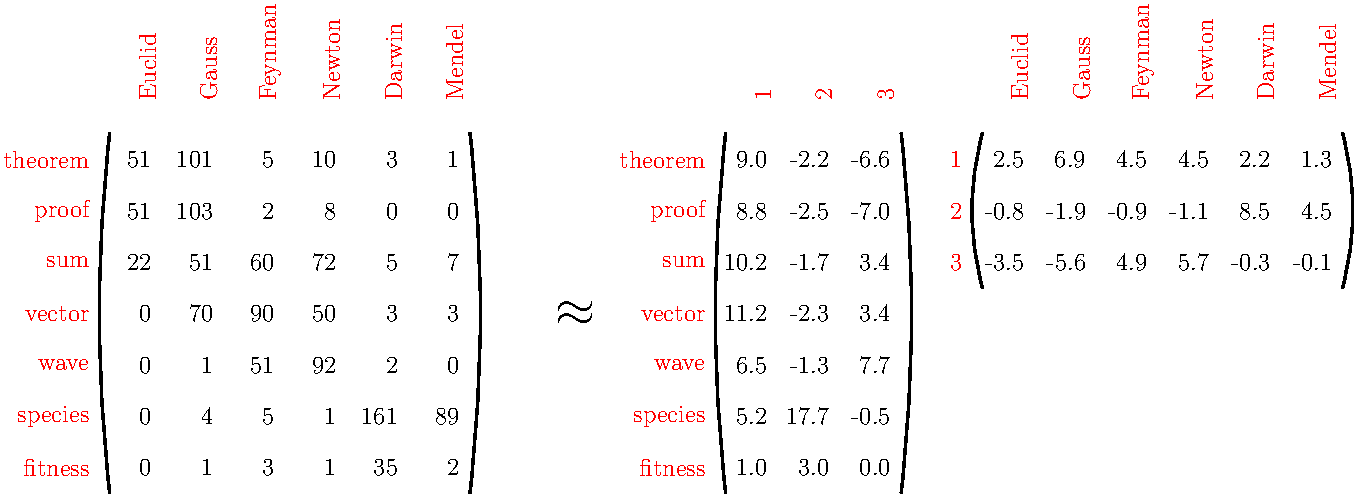
\includegraphics[width=\linewidth]{books}
\end{center}
\begin{itemize}
\item Best rank-3 approximation, but the factors mix signs: hard to
  interpret
\end{itemize}
\end{slide}

%%%%%%%%%%%%%%%%%%%%%%% Next Slide %%%%%%%%%%%%%%%%%%%%%%%

\begin{slide}
\section[-1]{Non-Negative Matrix Factorisation}

\begin{PauseHighLight}
  \begin{itemize}\squeeze
  \item When $\mat{X}$ is non-negative we can get a sparse model by
    minimising $E(\mat{A},\mat{B}) = \| \mat{X} - \mat{A}\,\mat{B}
    \|_F^2$ with all elements of $\mat{A}$ and $\mat{B}$ non-negative\pause
  \item Projected gradient descent: take a gradient step, then set
    negative elements to zero\pause
  \item Or Lee and Seung's \emph{multiplicative updates}
    ($\oslash$ is element-by-element division)
    \begin{align*}
      \mat{B} &\leftarrow \mat{B}\odot\bigl(\mat{A}^\tr\mat{X}\bigr)
                \oslash\bigl(\mat{A}^\tr\mat{A}\mat{B}\bigr), &
      \mat{A} &\leftarrow \mat{A}\odot\bigl(\mat{X}\mat{B}^\tr\bigr)
                \oslash\bigl(\mat{A}\mat{B}\mat{B}^\tr\bigr)
    \end{align*}
    which never make an element negative\pause
  \end{itemize}
\end{PauseHighLight}

\end{slide}

%%%%%%%%%%%%%%%%%%%%%%% Next Slide %%%%%%%%%%%%%%%%%%%%%%%

\begin{slide}
\section{Non-Negative Matrix Factorisation}
\begin{center}
  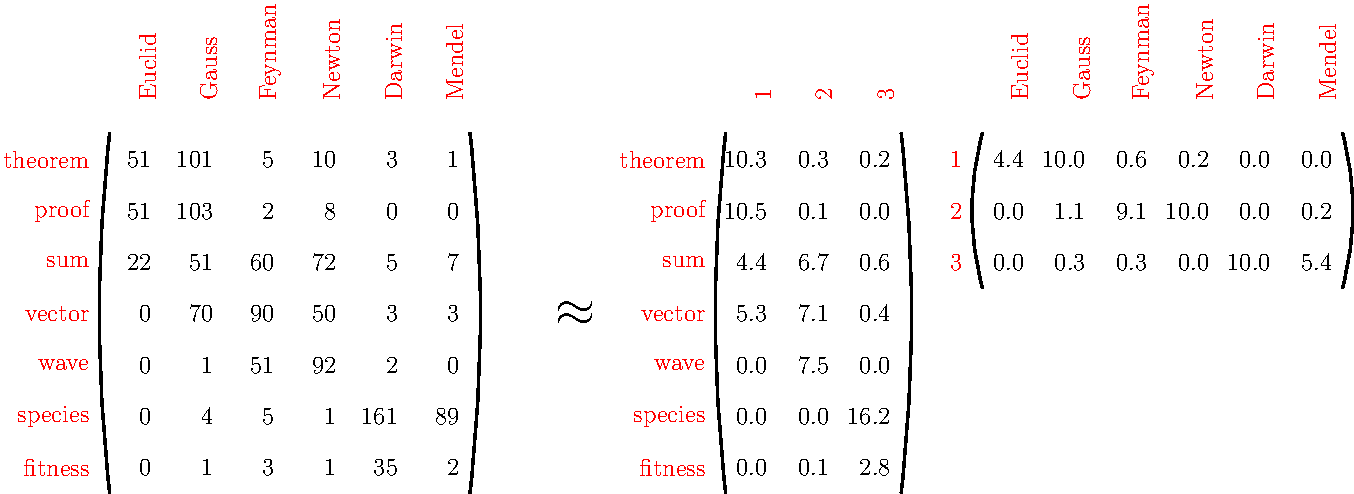
\includegraphics[width=\linewidth]{booksNN}\pause
\end{center}
\begin{itemize}
\item The three factors pick out mathematics, physics and
  biology\pauseb
\end{itemize}
\end{slide}

%%%%%%%%%%%%%%%%%%%%%%% Next Slide %%%%%%%%%%%%%%%%%%%%%%%

\begin{slide}
\section[-1]{Non-Negative Matrix Factorisation: Caveats}

\begin{PauseHighLight}
  \begin{itemize}
  \item NMF is very popular because its factors are often easier to
    interpret than those of the SVD\pause
  \item But
    \begin{itemize}
    \item It cannot fit better than the SVD: by Eckart--Young the
      truncated SVD is the best rank-$K$ fit\pause{} (here
      relative errors 0.164 against 0.158)\pause
    \item The problem is not convex: the answer depends on the
      starting point and on $K$\pause
    \item The factors are not unique, and a ``parts-based'' reading of
      them is not guaranteed\pause
    \end{itemize}
  \item Always compare against simple baselines (e.g. the SVD or
    PCA)\pause
  \end{itemize}
\end{PauseHighLight}

\end{slide}

%%%%%%%%%%%%%%%%%%%%%%% Next Slide %%%%%%%%%%%%%%%%%%%%%%%

\begin{slide}
\section{Conclusion}

\begin{PauseHighLight}
  \begin{itemize}
  \item Structured data typically lies close to a low-dimensional
    subspace, and we can exploit this\pause
  \item Matrix factorisation has many applications including recommender
    systems, data completion, and data modelling\pause
  \item The truncated SVD gives the best low-rank approximation;
    iterating it fills in missing entries\pause
  \item A Bayesian (MAP) approach helps with over-fitting, and each step
    of the resulting ALS is ridge regression\pause
  \item Non-negative matrix factorisation gives more interpretable,
    though not necessarily better, factors\pause
  \end{itemize}
\end{PauseHighLight}


\end{slide}

\end{document}

%% Imported 2026-10-20 from comp6208/old_lectures/matrix-completion.tex
%% and updated: low-rank theme, Eckart--Young, iterative SVD, ALS as ridge
%% regression, embeddings, NMF caveats.  Figures svdComplete and books are
%% generated by svdComplete.py and books.py (real numbers).
